\documentclass{note}
\usepackage[cpp,table]{mypackage}

\renewcommand{\thefootnote}{\fnsymbol{footnote}}

\title{操作系统原理笔记}
\author{陈鸿峥}
\date{{\builddatemonth\today}\protect\footnote{\text{Build \builddate\today}}} % protect!

\begin{document}

\maketitle
\renewcommand{\thefootnote}{\arabic{footnote}}
\setcounter{footnote}{0}

\setcounter{tocdepth}{2}%设置深度
\tableofcontents

\bigskip\bigskip
本课程使用的教材为William Stallings《操作系统---精髓与设计原理(第八版)》。
其他参考资料包括Stanford CS140、CMU15-460、\emph{Operating System Concepts (10th ed.)}。
\par 关于计算机系统的内容在此不再赘述,详情参见\textbf{计算机组成原理}的笔记。

% !TEX root = main.tex

\section{计算机系统概述}
\subsection{计算模型}
\begin{itemize}
	\item 图灵机(1936)
	\item 冯诺依曼体系结构(1945)\footnote{非冯诺依曼体系结构:并行计算、量子计算、生物计算} --- 存储程序原理(\textbf{运算器}为中心)\\
	计算机采用\textbf{二进制}表示机器指令和数据,按照程序指令\textbf{顺序}执行
\begin{center}
\begin{tikzcd}
& & \text{存储器}\arrow{d} & & \\
\quad\arrow{r} & \text{输入设备}\arrow{r} & \text{运算器}\arrow{r}\arrow{d}\arrow{u} & \text{输出设备}\arrow{r} & \quad\\
& & \text{控制器}\arrow{u}\arrow{lu}\arrow{ru}\arrow[bend left]{uu} & &
\end{tikzcd}
\end{center}
而现在由于计算不是瓶颈,存储访问成为了瓶颈,故现代微机以\textbf{存储器}为中心
\begin{center}
\begin{tikzcd}
& & \text{运算器}\arrow{d} & & \\
\quad\arrow{r} & \text{输入设备}\arrow{r} & \text{存储器}\arrow{r}\arrow{d}\arrow{u} & \text{输出设备}\arrow{r} & \quad\\
& & \text{控制器}\arrow{u}\arrow{lu}\arrow{ru}\arrow[bend left]{uu} & &
\end{tikzcd}
\end{center}
\end{itemize}
[运算器、控制器](CPU)、存储器为计算机的核心,合称主机;外围设备,简称外设,指除主机外的其他设备,包括IO设备、外存等

计算机中的信息仍用二进制表示的原因:由物理器件性能决定
\begin{itemize}
	\item 二进制只有两种状态,容易找到具有2个稳定状态并且状态转换容易控制的物理器件(数字电路)
	\item 二进制编码运算规则简单
	\item 二进制的0、1与二值逻辑一致,容易实现逻辑运算
\end{itemize}
% There are two reasons computers use the binary system:
% 1.Two clearly distinct states that provide a safety range for reliability.
% 2.Least amount of necessary circuitry, which results in the least amount of space, energy consumption, and cost.

\subsection{计算机的发展历程}
按发展历程可分为:电子管、晶体管、集成电路、(超)大规模集成电路四代计算机
\par重大历史事件如下
\begin{center}
\begin{tabular}{|c|c|c|c|}
\hline
% 年份 & 姓名 & 事件 & 备注 \\
1904 & 弗莱明(Fleming) & 二极管 & \\\hline
1907 & 德福雷斯特(De Forest) & 三极管 & \\\hline
1938 & 香农(Shannon) & 布尔代数与二值电子器件(继电器) & 奠定数字电路基石 \\\hline
1946 & & 第一台通用计算机ENIAC & 十进制 \\\hline
1947 & \begin{tabular}{c}布莱顿(Brattain)\\
巴丁(Bardeen)\end{tabular} & 点接触晶体管 & \\\hline
1949 & 肖克利(Shockley) & 结型晶体管(1949) & 1956诺贝尔奖\\\hline
1950 & & 二进制和存储程序EDVAC & 实现冯诺依曼设想(组合进步) \\\hline
1958 & Jack Kilby & 集成电路 & 2000诺贝尔奖 \\\hline
1965 & Moore & 摩尔定律 & \begin{tabular}{c}
在价格不变的情况下,每18个月芯片上\\
晶体管数目翻倍,性能也提升一倍
\end{tabular}\\\hline
1971 & Intel & 第一款微处理器4004 & 10$\mu$m\\\hline
\end{tabular}
\end{center}

\subsubsection{单处理器(1971-2002)}
性能提升主要手段
\begin{itemize}
	\item 提升工作主频:KHz增长至GHz(生产工艺进步,流水线级数增加)
	\item 指令级并行(ILP)
\end{itemize}
\begin{proposition}[安迪-比尔定律]
Andy gives, Bill takes away. 安迪是原Intel CEO,比尔是原微软CEO,硬件厂商靠软件开发商用光自己提供的硬件资源得以生存
\end{proposition}
但遇到频率墙和功耗墙
\[\text{功耗(power)}\propto 1/2\times\text{CMOS电容}\times\text{电压}^2\times\text{转换(01)频率}\]
\par
2004年,Intel放弃4GHz Pentium4芯片开发,因无法解决散热问题,通过加快主频提升处理器性能的路走到尽头

\subsubsection{多核处理器(2005-)}
采用多核处理器不过是将硬件的问题丢到软件\footnote{“向多核的转变并不是因为我们在软件或体系结构技术上取得了中大突破而带来的。相反,这种转变是当单处理器体系结构发展遇到了难以克服的巨大障碍时,我们被迫作出的一种选择。”---Kurt Keutzer (UCB), \emph{The Landscape of Parallel Computing Research: A View from Berkeley}}
\begin{theorem}[阿姆达尔(Amdahl)定律]
\label{thm:amdahl}
\[\text{改进后的执行时间}=\text{受改进影响部分的执行时间}/\text{改进提高的倍数}+\text{不受影响的执行时间}\]
\[S_A=\frac{1}{s+(1-s)/N},\]
\end{theorem}
对计算机系统的某个部分采用并行优化措施后所获得的计算机性能的提高是有上限的,上限由串行部分所占的比例决定
\begin{theorem}[古斯塔夫森(Gustafson)定律]
\[S_G=(s'+p'\times N)/(s'+p')=N+(1-N)\times s',\]
其中,$s'$和$p'$为程序串行部分与可并行化部分在并行系统上执行的时间占总时间的比例,$N$为处理器数量,简便起见设总时间$s'+p'=1$
\end{theorem}
打破Amdahl定律\textbf{问题规模不变}的假设,任何足够大的任务都可以被有效地并行化,只要问题规模可扩展,并行所带来的加速比就可以扩展


\subsection{计算机系统的层次结构}
\begin{center}
\begin{tikzcd}
\text{高级语言层}\arrow{d}{}\\
\text{汇编语言层}\arrow{d}{}\\
\text{操作系统层}\arrow{d}{}\\
\text{指令系统层}\arrow{d}{}\\
\text{微体系结构层}\arrow{d}{}\\
\text{数字逻辑层}
\end{tikzcd}
\end{center}
程序编译运行过程:
\begin{center}
\begin{tikzcd}
\text{高级语言}\quad\arrow{r}{\text{预编译、编译}} & \quad\text{汇编语言}\arrow{r}{\text{汇编}} & \text{目标文件(二进制)}\arrow{r}{\text{链接}} & \text{可执行文件(二进制)}\arrow{d}{\text{加载}}\\
& & \text{电路上的电信号}\quad & \quad\text{二进制机器指令流(硬盘$\to$存储器)}\arrow[swap]{l}{\text{CPU取指译码}}
\end{tikzcd}
\end{center}
计算机内部工作过程:逐条执行加载到内存中的二进制机器指令流的过程

指令执行分为两个阶段,周期性重复性进行:
\begin{itemize}
	\item 取指阶段:CPU从内存中读取指令,程序计数器(PC)保存要被要被取出的\textbf{下一条}指令的地址,除非遇跳转指令,否则都加一个增量\footnote{程序计数器(Program Counter)是一个实际存在的寄存器吗? - Belleve的回答 - 知乎 \url{https://www.zhihu.com/question/22609253/answer/21965180} PC每次增加\textbf{一条指令的长度/寻址粒度},在MIPS中一条指令长4字节,寻址粒度1字节,故每次PC加4;而x86体系指令长度不定,每次增加量会变化}
	\item 执行阶段:对取出的指令译码后执行
\end{itemize}
软件系统可分为系统软件和应用软件

\subsection{计算机结构的八个想法}
\begin{enumerate}
	\item 摩尔(Moore)定律:集成电路资源每$18-24$个月翻倍
	\item 抽象(abstraction):简化设计
	\item 加速常用操作(Make common case fast):见定理\ref{thm:amdahl}
	\item 并行(parallelism)
	\item 流水线(pipelining)
	\item 预测(prediction)
	\item 内存等级制(hierarchy)
	\item 冗余实现可靠性(redundancy):检测故障及解决
\end{enumerate}

\subsection{基本指标}
表示计算机通信带宽时
\begin{center}
\begin{tabular}{ccccccc}\hline
KB(yte) & MB & GB & TB & PB & EB & ZB\\\hline
$10^3$ & $10^6$ & $10^9$ & $10^{12}$ & $10^{15}$ & $10^{18}$ & $10^{21}$\\\hline
\end{tabular}
\end{center}
表示计算机存储二进制时
\begin{center}
\begin{tabular}{ccccccc}\hline
KiB(yte) & MiB & GiB & TiB\\\hline
$2^{10}$ & $2^{20}$ & $2^{30}$ & $2^{40}$\\\hline
\end{tabular}
\end{center}
\begin{itemize}
	\item 位(bit/b):计算机处理、存储、传输信息的最小单位
	\item 字节(Byte/B) $1\text{ Byte}=8\text{ bit}$:现代计算机主存按字节编制,字节是最小可寻址单位
	\item 字(Word):表示被处理信息的单位,用来度量数据类型的宽度\footnote{字长是指CPU中\textbf{数据通路的宽度},等于CPU内部总线的宽度或运算器的位数或通用寄存器的宽度;字和字长的宽度可以一样,也可以不同,通常是字节的整数倍}
\end{itemize}
\par 一台32位的电脑,一个字等于4个字节,字长为32位;若字长为16位,则一个字等于2字节.
\par 4字节相当于8位16进制编码

\subsection{性能评价}
\label{subsec:performance}
CPU主频:对同一型号计算机,主频越高,完成指令一个执行步骤时间越短
\[\text{计算机的性能(Performance)}=1/\text{执行时间(Execution time)}\]
按照单位(量纲)进行换算即可
\[\begin{aligned}
\text{CPU执行时间(s)}&=\text{执行程序所需CPU时钟周期(cyc)}\times\text{时钟周期s/cyc)}\\
&=\text{指令数目(ins)}\times\text{CPI(cyc/ins)}\times\text{时钟周期(s/cyc)}
\end{aligned}\]
程序性能对执行事件的影响:
\begin{center}
\begin{tabular}{|c|c|c|c|}\hline
 & 指令数 & CPI & 时钟周期\\\hline
算法、编程语言、编译器 & $\times$ & $\times$ & \\\hline
指令集 & $\times$ & $\times$ & $\times$ \\\hline
计算机组成 & & $\times$ & $\times$ \\\hline
实现技术 & & & $\times$\\\hline
\end{tabular}
\end{center}
体系结构=指令集体系结构(功能定义与设计)+计算机组成(考虑用什么材料)\\
举例来说:
\begin{itemize}
	\item 指令集(ISA)考虑:是否提供乘法指令
	\item 组成(Organization)考虑:如何实现乘法指令(专门乘法器还是加法器+移位器)
	\item 实现技术(Technology)考虑:如何布线、用什么材料和工艺
\end{itemize}

% 带有处理器的设备一般称为智能化设备
% 完整的计算机系统应包括配套的硬件设备和软件系统
% !TEX root = main.tex

\section{进程}
进程(process)是\textbf{运行时(running/in execution)}程序的实例。
\begin{itemize}
	\item 程序并发执行的特征(多道程序):间断性、无封闭性、不可再现性(破环冯顺序执行特性)
	\item 进程的特点:动态性、并发性、独立性、异步性
	\item 进程的作用
	\begin{itemize}
		\item 提升CPU利用率:将多个进程重叠(一个进程IO时另一个计算)
		\item 降低延迟(latency):并发执行,不断切换,防止卡住
	\end{itemize}
\end{itemize}

进程控制块(Process Control Block, PCB),在Unix是proc,在Linux是task\_struct
\begin{itemize}
	\item 进程标识符/ID
	\item 五状态:运行、就绪、等待/阻塞、创建、结束
	\begin{figure}[H]
	\centering
	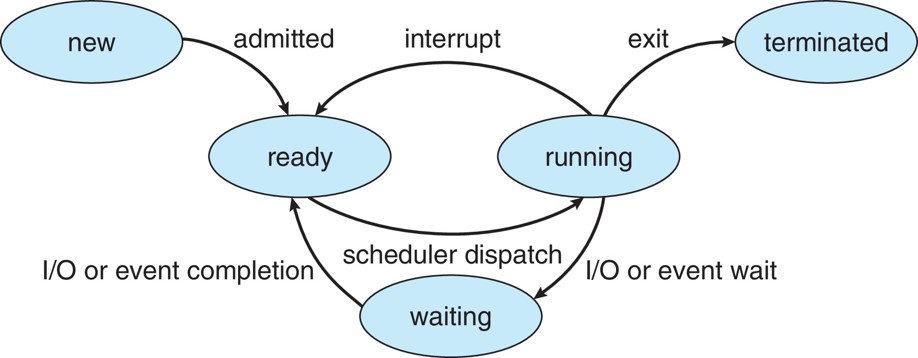
\includegraphics[width=0.6\linewidth]{fig/5-state-process-model.jpg}
	\end{figure}
	\item 优先级
	\item 程序计数器(PC)
	\item 内存指针:报错指向程序代码、相关数据和共享内存的指针
	\item 上下文数据(context):进程被中断时寄存器中的数据
	\item IO状态信息
	\item 记账信息(accounting):占用处理器时间、时钟数总和、时间限制等
	\item 链表:各状态的进程形成不同的链表:就绪链表、阻塞链表等
\end{itemize}

% 如果想要进程之间交互,则通过文件进行,如sublime编辑文件,gcc对其进行编译
进程间的通信
\begin{itemize}
	\item 共享存储:进程到共享空间再到进程
	\item 消息传递:直接进程到进程
	\item 管道通信:进程到缓冲区到进程,管道即共享文件,半双工通信
\end{itemize}

进程控制由原语(primitive)完成,由若干条指令完成,也可被视为原子操作

内存组织:代码段、数据段、堆段、栈段(从小地址往大地址)
\begin{figure}[H]
\centering
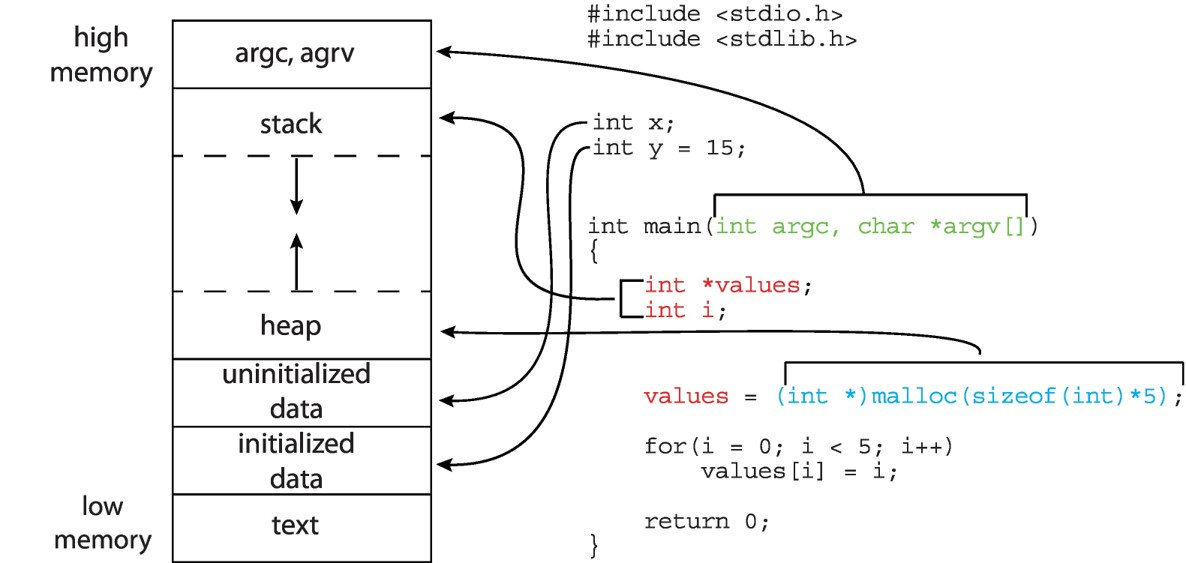
\includegraphics[width=0.8\linewidth]{fig/C_memory.jpg}
\end{figure}

可以参考原始的UNIX论文\footnote{\url{http://www.scs.stanford.edu/19wi-cs140/sched/readings/unix.pdf}}。
\begin{itemize}
	\item 创建进程:fork、waitpid
	\item 删除进程:exit、kill
	\item 执行进程:execve
\end{itemize}

% COM 基于组件共享技术 软件重用
% OLE

% 可再入/不可再入内核

处理器上下文即处理器寄存器的内容
\begin{center}
\begin{tikzcd}
\text{就绪}\arrow[bend left]{rr}{\text{分派}} & & \text{运行}\arrow[bend left]{ll}{\text{超时}}
\end{tikzcd}
\end{center}

% shell:用户控制台,解释用户指令

导致OS获得控制权的事件:
\begin{itemize}
	\item 时钟中断:时间片结束
	\item IO中断:IO完成
	\item 硬件中断/陷阱(trap)/异常
	\item 系统调用:\verb'int'
\end{itemize}
% !TEX root = main.tex

\section{线程}
在没有线程概念的系统中,进程是\textbf{资源分配}、调度/执行的单位;而在有线程概念的系统中,线程就成了\textbf{基本调度单位}/程序执行流最小单元,由线程ID、程序计数器、寄存器集合和堆栈组成。

线程的优点:
\begin{itemize}
    \item 创建速度快
    \item 终止所用时间少
    \item 切换时间少
    \item 通信效率高,同一进程无需调用内核,共享存储空间
\end{itemize}

\bigskip
用户级线程(ULT):线程管理都由应用程序完成(线程库),内核不知道线程的存在,优点:
\begin{itemize}
    \item 线程切换不需要模式切换
    \item 调度算法可以应用程序专用
    \item ULT不需要内核支持,线程库可以在任何OS上运行
\end{itemize}
缺点:
\begin{itemize}
    \item 一个线程阻塞会导致整个进程阻塞
    \item 不能利用多核和多处理器技术
\end{itemize}

\bigskip
内核级线程(KLT):线程管理由内核完成(提供API),调度基于线程进行,优点:
\begin{itemize}
    \item 线程阻塞不会导致进程阻塞
    \item 可以利用多核和多处理器技术
    \item 内核例程本身也可以使用多线程
\end{itemize}
缺点:
\begin{itemize}
    \item 线程切换需要进行模式切换
\end{itemize}

\bigskip
多线程模型
\begin{itemize}
    \item 多对一:多个用户级线程映射到一个内核级线程,线程管理在用户空间进行,效率高;若内核服务阻塞,则整个进程被阻塞
    \item 一对一:每个用户级线程映射到一个内核级线程,开销大
    \item 多对多:折中
\end{itemize}
\begin{figure}[H]
    \centering
    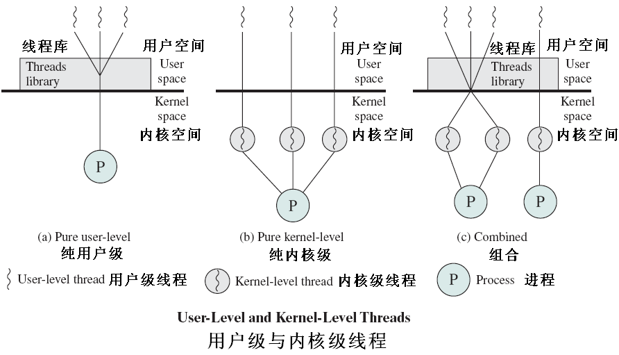
\includegraphics[width=0.6\linewidth]{fig/threads.png}
\end{figure}

线程与进程之间的关系
\begin{itemize}
    \item 1:1,每个进程都有唯一线程,DOS、传统Unix
    \item M:1,一个进程多个线程,Windows NT、Linux、Mac OS、iOS
    \item 1:M,一个线程可在多个进程环境中迁移
\end{itemize}

* Linux并不区分线程和进程,采用Copy On Write (COW)方式
% !TEX root = main.tex

\section{并发---互斥与同步}
\subsection{基本概念}
\begin{itemize}
    \item 原子(atomic)操作:不可分割
    \item 临界区(critical section):不允许多个进程同时进入的一段访问\textbf{共享资源}的代码
    \item 死锁(deadlock):两个及以上进程,因每个进程都在等待其他进程做完某事(如释放资源),而不能继续执行
    \item 活锁(livelock):两个及以上进程,为响应其他进程中的变化,而不断改变自己的状态,但是没有做任何有用的工作
    \item 互斥(mutual exclusion):当一个进程在\textbf{临界区访问共享资源}时,不允许其他进程进入访问
    \item 竞争条件(race condition, RC):多个进程/线程读写共享数据,其结果依赖于它们执行的相对速度
    \item 饥饿(starvation):可运行的进程长期未被调度执行
\end{itemize}

核心内容
\[\text{并发}\to\text{共享}\to\text{RC问题}\to\text{互斥}\]

共享数据的最终结果取决于进程执行的相对速度(异步性),需要保证进程的结果与相对执行速度无关

同步:有明确的时间先后限制,两个或多个进程之间的操作存在时间上的约束(也包含互斥)

\subsection{互斥}
互斥的要求
\begin{itemize}
    \item 在具有相同资源或共享对象的临界区的所有进程中,一次只允许一个进程进入临界区(强制排它)
    \item 一个在非临界区停止的进程必须不干涉其他进程(充分并发)
    \item 没有进程在临界区中时,任何需要访问临界区的进程必须能够立即进入(空闲让进)
    \item 决不允许出现一个需要访问临界区的进程被无限延迟(有限等待)
    \item 相关进程的执行速度和处理机数目没有任何要求或限制(满足异步)
    \item 当进程不能进入临界区,应该立即释放处理机,防止进程忙等待(让权等待)
\end{itemize}

\subsubsection{简单的尝试}
第一种尝试(单标志法):两个进程轮流进入临界区

\begin{minipage}{0.5\linewidth}
\begin{lstlisting}
while (turn != 0)
    /* do nothing */;
/* critical section */
turn = 1;
\end{lstlisting}
\end{minipage}
\begin{minipage}{0.5\linewidth}
\begin{lstlisting}
while (turn != 1)
    /* do nothing */;
/* critical section */
turn = 0;
\end{lstlisting}
\end{minipage}

可以保证互斥,硬性规定进入的顺序,但是
\begin{itemize}
    \item 忙等待,白白消耗CPU时间
    \item 必须轮流进入临界区,不合理,限制推进速度
    \item 若一个进程失败,则另一个将永远被阻塞
\end{itemize}
难以支持并发处理

一共四种尝试
\begin{itemize}
    \item 单标志法
    \item 双标志先检查:死锁
    \item 双标志后检查:不能保证互斥
    \item 双标志延迟礼让:活锁
\end{itemize}

\subsubsection{软件方法}
Dekker算法:避免无原则礼让,规定各进程进入临界区的顺序;逻辑复杂,正确性难以证明,存在轮流问题,存在忙等待;初始化\verb'flag'都为\verb'false',\verb'turn'为1
% https://www.cnblogs.com/zhengruin/p/4994188.html
\begin{lstlisting}
void P0()
{
	while(true)
	{
		flag[0] = true; // `P0想使用关键区'
		while(flag[1]) // `检查P1是不是也想用?'
		{
			if(turn == 1) // `如果P1想用,则查看P1是否具有访问权限?'
			{
				flag[0] = false; // `如果有,则P0放弃'
				while(turn == 1); // `检查turn是否属于P1'
				flag[0] = true; // `P0想使用'
			}
		}
		visit(0); // `访问Critical Partition'
		turn = 1; // `访问完成,将权限给P1'
		flag[0] = false; // `P0结束使用'
	}
}

void P1()
{
	while(true)
	{
		flag[1] = true; // `P1想使用关键区'
		while(flag[0]) // `检查P0是不是也想用?'
		{
			if(turn == 0) // `如果P0想用,则查看P0是否具有访问权限?'
			{
				flag[1] = false; // `如果有,则P1放弃'
				while(turn == 0); // `检查turn是否属于P1'
				flag[1] = true; // ` P1想使用'
			}

		}
		  visit(1); // `访问Critical Partition'
		turn = 0; // `访问完成,将权限给P0'
		flag[1] = false; // `P1结束使用'
	}
}
\end{lstlisting}

Peterson算法:flag和turn的含义同Dekker的,但先设turn=别人,且只有flag[别人]和turn=别人同时为真时才循环等待
\begin{lstlisting}
void P0()
{
        while(true)
        {
                flag[0] = true;
                turn = 1;
                while(flag[1] && turn == 1)
                // `退出while循环的条件就是,要么另一个线程'
                // `不想要使用关键区,要么此线程拥有访问权限'
                {
                        sleep(1);
                        printf("procedure0 is waiting!\n");
                }
                //critical section
                flag[0] = false;
        }
}

void P1()
{
        while(true)
        {
                flag[1] = true;
                turn = 0;
                while(flag[0] && turn == 0)
                {
                        sleep(1);
                        printf("procedure1 is waiting!\n");
                }
                //critical section
                flag[1] = false;
        }
}
\end{lstlisting}

\subsubsection{硬件方法}
\begin{itemize}
    \item 关中断:限制处理器交替执行各进程的能力,不能用于多核
    \item 专用指令:\textbf{比较并交换},原子指令,一个指令周期内完成,不会被中断
    \begin{itemize}
        \item TestSet(TS)指令,比较并交换的bool形式
\begin{lstlisting}
int compare_and_swap (int *word, int testval, int newval)
bool testset (int i)
\end{lstlisting}
        \item Exchange/swap指令(x86\verb'xchg'指令):同上,适用于单核多核,多变量多临界区,但需要忙等待(busy waiting)/自旋等待(spin waiting),可能饥饿或死锁
\begin{lstlisting}
void exchange (int register, int memory)
\end{lstlisting}
    \end{itemize}
\end{itemize}

机器指令方法优点
\begin{itemize}
    \item 适用于单处理器或共享主存多[核]处理器系统,进程数目任意
    \item 简单且易于证明
    \item 可以使用多个变量支持多个临界区
\end{itemize}
缺点
\begin{itemize}
    \item 忙等待/自旋等待
    \item 可能饥饿或死锁
\end{itemize}

\subsection{信号量(semaphore)}
解决RC问题一种简单高效的方法

\subsubsection{基本操作}
记录信号量
\begin{itemize}
    \item 整数:可用资源数($\geq 0$),需要初始化
    \item P操作(proberen,\verb'semWait'):信号量的值\textbf{减1}(申请一个单位的资源),若信号量变为\textbf{负数},则执行P操作进程阻塞,\textbf{让权等待}
    \item V操作(verhogen,\verb'semSignal'):信号量的值\textbf{加1}(释放一个单位的资源),若信号量\textbf{不是正数}(绝对值=现被阻塞的进程数/等待队列的长度),则使一个因P操作被阻塞的进程解除阻塞(唤醒)
\end{itemize}
需要保证P操作和V操作的\textbf{原子性}!
\begin{lstlisting}
struct semaphore {
    int count;
    struct process* L; // `阻塞队列'
} s;
void P(semaphore s) { // semWait
    s.count--;
    if (s.count < 0)
        Block(CurruntProcess, s.L);
        // `将当前进程插入该信号量对应的阻塞队列'
}
void V(semaphore s) { // semSignal
    s.count++;
    if (s.count <= 0)
        WakeUp(s.L);
}
\end{lstlisting}
注意P操作是\textbf{小于0},V操作\textbf{小于等于0}\footnote{理解为先判断是否小于0(阻塞队列非空),然后再++会比较好},且一个进程只会在一个信号量的阻塞队列中。

信号量的优点是简单且表达能力强,用P、V操作可解决多种类型的同步/互斥问题,但不够安全,P、V操作使用不当会产生死锁。

二元信号量省空间,不能代表资源数量,要引入全局变量代表数量。

\subsubsection{实现互斥(mutex)}
\begin{itemize}
    \item 对于每一个RC问题,设一个信号量(向系统调用/向内核调用),\textbf{初始化为$1$}
    \item 所有相关进程在进入临界区\textbf{之前}对该信号量进行\textbf{P操作}
    \item 出临界区\textbf{之后}进行\textbf{V操作}
\end{itemize}

\subsubsection{同步}
同步:后续动作必须在前驱动作执行完后才能进行
\begin{itemize}
    \item 对每一个同步关系都要设一个信号量,初值看具体问题(一般为0)
    \item 在\textbf{前驱动作之后}执行V操作(相当于资源产生了)
    \item 在\textbf{后续动作之前}执行P操作
\end{itemize}

\subsubsection{生产者-消费者问题}
\begin{lstlisting}
void producer() {
    while (true) {
        produce();
        P(e);

        P(s);
        append();
        V(s);

        V(n); // first
    }
}

void consumer() {
    while (true) {
        P(n); // after

        P(s);
        take();
        V(s);

        V(e);
        consume();
    }
}

// s = initSem(1); // mutex
// n = initSem(0); // # products
// e = initSem(12); // # empty entries in buffer
\end{lstlisting}

\subsubsection{读者写者问题}
可以有多个读者,但只有一个写者

读者优先
\begin{lstlisting}
int readcount;
semaphore x=1, wsem=1;
void reader() {
    while(true) {
        P(x);
        readcount++;
        if (readcount==1) P(wsem);
        V(x);
        READUNIT();
        P(x);
        readcount--;
        if (readcount==0) V(wsem);
        V(x);
    }
}

void writer() {
   while(true) {
       P(wsem);
       WRITEUNIT();
       V(wsem);
   }
}
\end{lstlisting}

写者优先
\begin{lstlisting}[multicols=2]
int readcount, writecount;
semaphore x=1, y=1, z=1, rsem=1, wsem=1;
void reader() {
    while(true) {
        P(z); P(rsem);
        P(x);
        readcount++;
        if (readcount==1) P(wsem);
        V(x);
        V(rsem); V(z);
        READUNIT();
        P(x);
        readcount--;
        if (readcount==0) V(wsem);
        V(x);
    }
}

void writer() {
    while(true) {
        P(y);
        writecount++;
        if (writecount==1) P(rsem);
        V(y);
        P(wsem);
        WRITEUNIT();
        V(wsem);
        P(y);
        writecount--;
        if (writecount==0) V(rsem);
        V(y);
    }
}
\end{lstlisting}

\subsection{管程(monitor)}
管程(monitor):通过集中管理(封装同步机制与同步策略)以保证安全(类似于OOP中的抽象类)

主要特点:
\begin{itemize}
    \item 本地变量只能由管程过程访问(封装)
    \item 进程通过调用管程过程进入管程(调用)
    \item 每次只能一个进程在执行相关管程的过程(互斥)
\end{itemize}
主要缺陷
\begin{itemize}
    \item 可能增加了两次多余的进程切换
    \item 对进程调度有特殊要求(不允许插队)
\end{itemize}

\subsection{消息传递}
send和receive。

同样可以实现互斥,相当于在进程间传递一个可使用临界区的令牌
% !TEX root = main.tex

\section{并发---死锁与饥饿}
\subsubsection{死锁}
死锁(deadlock):一个进程集合中的每个进程都在等待只能由该集合中的其他一个进程才能引发的事件(释放占有资源/进行某项操作)
\begin{figure}[H]
    \centering
    \begin{tabular}{c}
    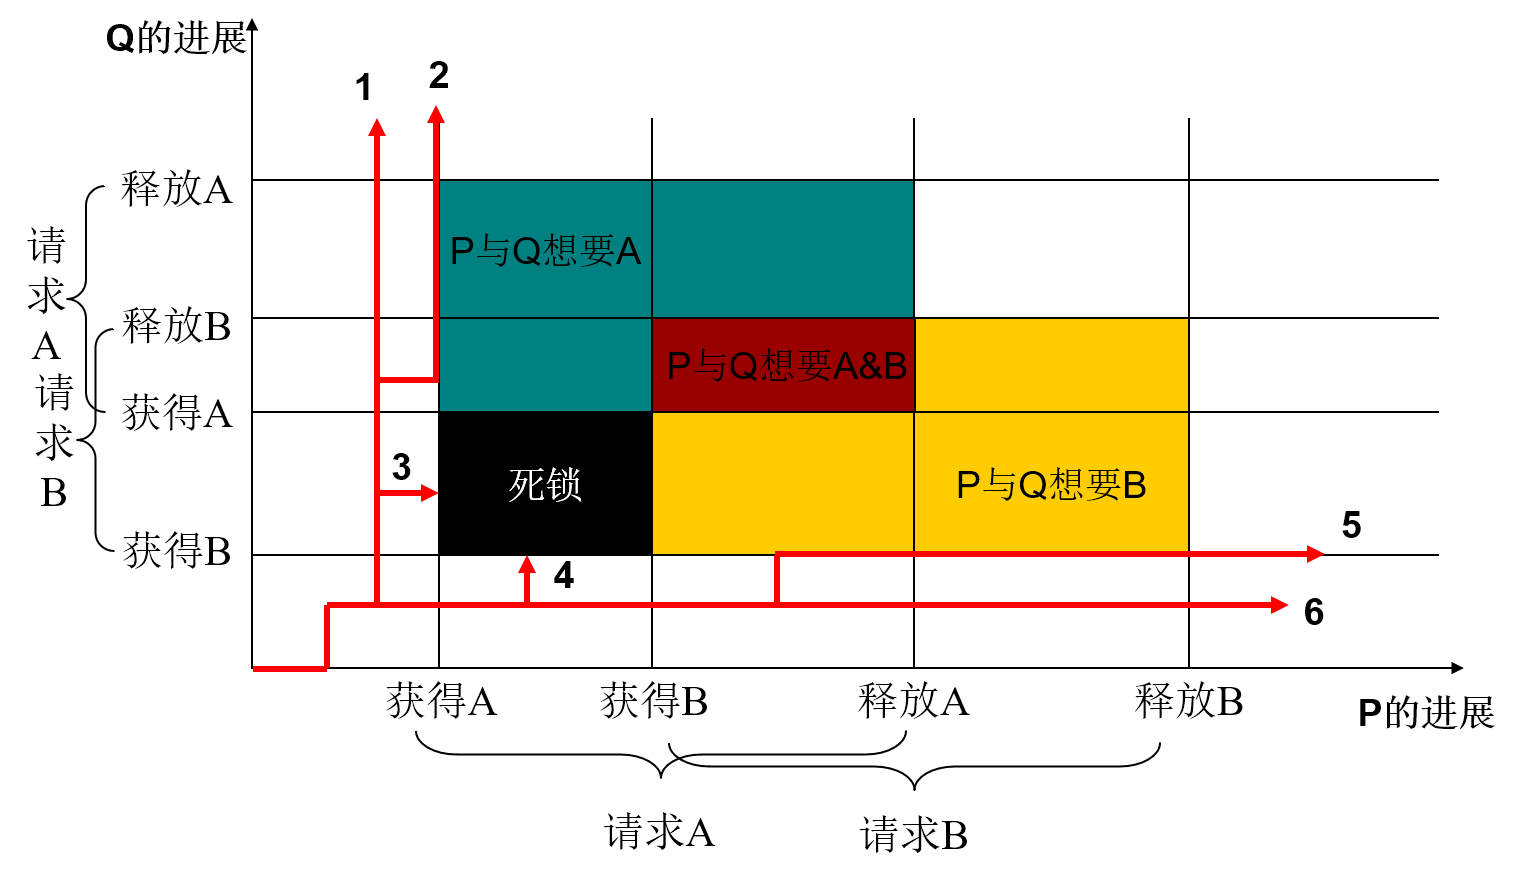
\includegraphics[width=0.8\linewidth]{fig/deadlock.png}\\
    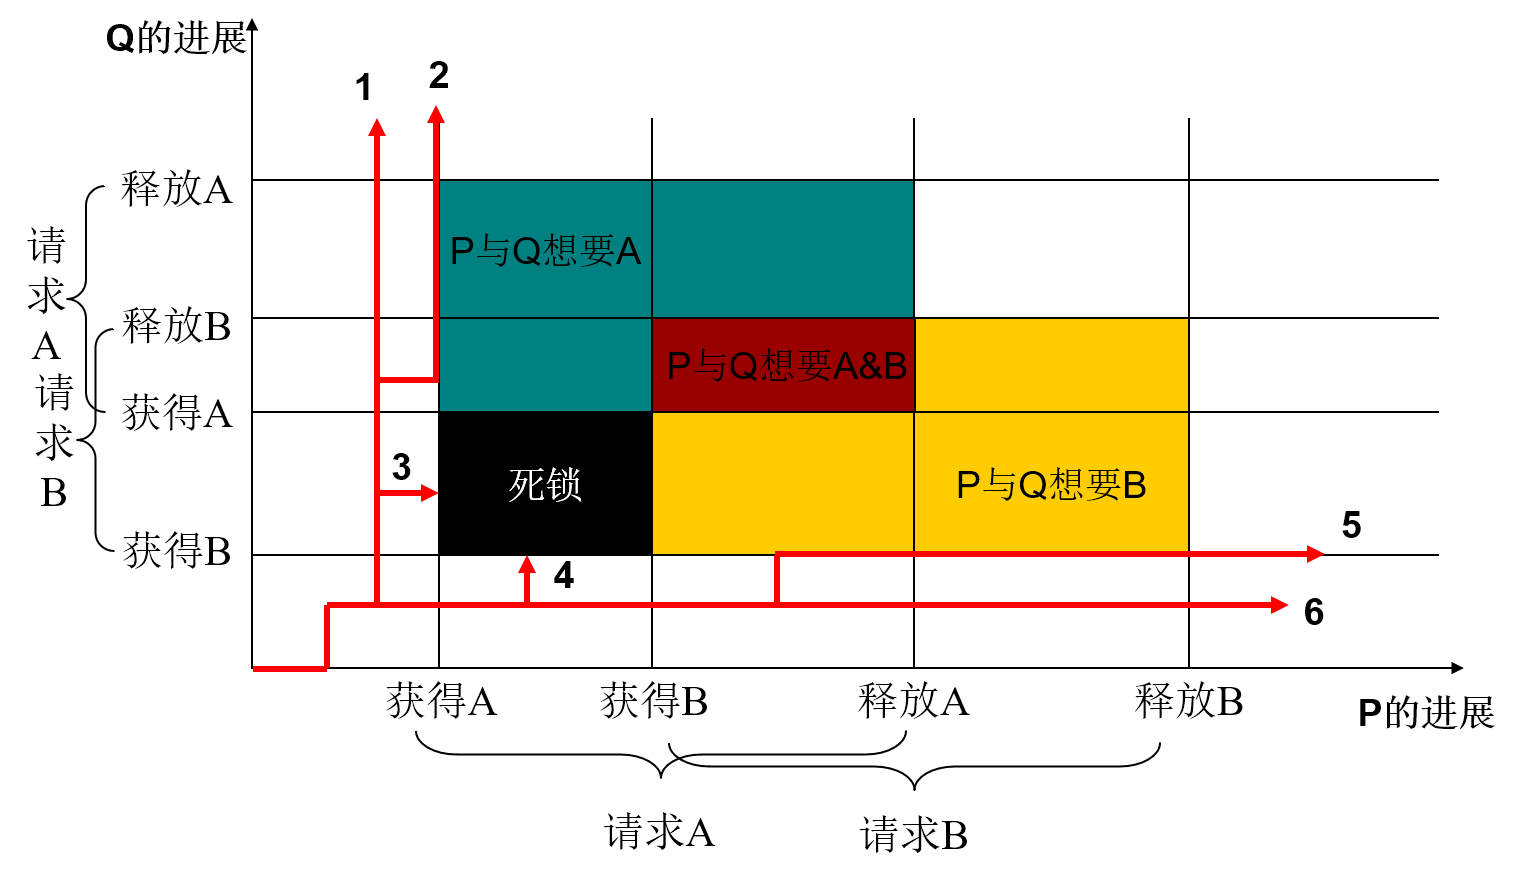
\includegraphics[width=0.8\linewidth]{fig/deadlock.png}
    \end{tabular}
    \caption*{联合进程图,上图死锁,下图无死锁}
\end{figure}

\begin{center}
\begin{tabular}{|l|l|l|p{10em}|l|}
\hline
\multicolumn{1}{|p{3.065em}|}{原则} & \multicolumn{1}{p{6em}|}{资源分配策略} & \multicolumn{1}{p{10em}|}{不同的方案} & 主要优点  & \multicolumn{1}{p{10em}|}{主要缺点} \bigstrut\\
\hline
\multicolumn{1}{|l|}{\multirow{6}[6]{*}{预防}} & \multicolumn{1}{l|}{\multirow{6}[6]{*}{保守,预提交(undercommits)资源}} & \multicolumn{1}{l|}{\multirow{3}[2]{*}{一次性请求所有资源}} & \tabitem对执行单一突发行为的进程有效 & \multicolumn{1}{p{10em}|}{\tabitem低效} \bigstrut[t]\\
      &       &       & \tabitem不需抢占 & \multicolumn{1}{p{10em}|}{\tabitem延时进程的初始化} \\
      &       &       & \multicolumn{1}{r|}{} & \multicolumn{1}{p{10em}|}{\tabitem进程必须知道未来的资源请求} \bigstrut[b]\\
\cline{3-5}      &       & \multicolumn{1}{p{10em}|}{抢占} & \tabitem便于用于状态易保存和恢复的资源 & \multicolumn{1}{p{10em}|}{\tabitem过多的不必要抢占} \bigstrut\\
\cline{3-5}      &       & \multicolumn{1}{l|}{\multirow{2}[2]{*}{资源排序}} & \tabitem通过编译时检测可实施 & \multicolumn{1}{l|}{\multirow{2}[2]{*}{\tabitem不允许增加资源请求}} \bigstrut[t]\\
      &       &       & \tabitem由于问题已在系统设计时解决,不需运行时再计算 &  \bigstrut[b]\\
\hline
\multicolumn{1}{|l|}{\multirow{2}[2]{*}{避免}} & \multicolumn{1}{l|}{\multirow{2}[2]{*}{位于检测和预防中间}} & \multicolumn{1}{l|}{\multirow{2}[2]{*}{操纵以发现至少一条安全路径}} & \multirow{2}[2]{*}{\tabitem不需抢占} & \multicolumn{1}{p{10em}|}{\tabitem OS必须知道未来的资源请求} \bigstrut[t]\\
      &       &       & \multicolumn{1}{l|}{} & \multicolumn{1}{p{10em}|}{\tabitem进程可能被长期阻塞} \bigstrut[b]\\
\hline
\multicolumn{1}{|l|}{\multirow{2}[2]{*}{检测}} & \multicolumn{1}{l|}{\multirow{2}[2]{*}{非常自由;尽可能地准许请求的资源}} & \multicolumn{1}{l|}{\multirow{2}[2]{*}{周期性地调用以测试死锁}} & \tabitem不会延时进程的初始化 & \multicolumn{1}{l|}{\multirow{2}[2]{*}{\tabitem丢失固有抢占}} \bigstrut[t]\\
      &       &       & \tabitem易于在线处理 &  \bigstrut[b]\\
\hline
\end{tabular}%
\end{center}

死锁定理:资源分配图中存在环路是存在死锁的充分必要条件
\begin{figure}[H]
    \centering
    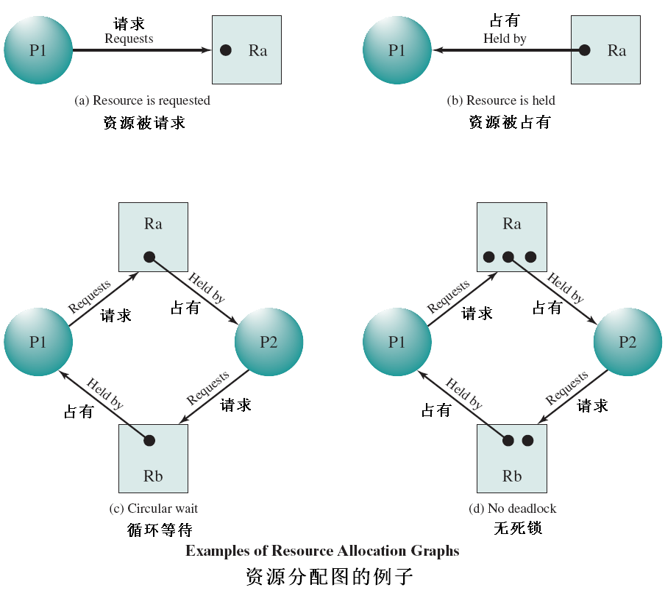
\includegraphics[width=0.6\linewidth]{fig/resource_graph.png}
\end{figure}

死锁的充分必要条件
\begin{itemize}
    \item 互斥
    \item 占有且等待
    \item 不可抢占
    \item 循环等待
\end{itemize}

\subsection{死锁预防}
破坏互斥条件:允许多个进程同时使用资源,但不适用于绝大多数资源

适用条件
\begin{itemize}
\item 资源的固有特性允许多个进程同时使用(如文件允许多个进程同时读)
\item 借助特殊技术允许多个进程同时使用(如打印机借助Spooling技术)
\end{itemize}

破坏占有且等待条件:禁止已拥有资源的进程再申请其他资源,如要求所有进程在开始时一次性地申请在整个运行过程所需的全部资源;或申请资源时要先释放其占有资源后,再一次性申请所需全部资源
\begin{itemize}
    \item 优点:简单、易于实现、安全
    \item 缺点:进程延迟运行,资源严重浪费
\end{itemize}

破坏不可剥夺条件:一个已经占有了某些资源的进程,当它再提出新的资源请求而不能立即得到满足时,必须释放它已经占有的所有资源,待以后需要时再重新申请;OS可以剥夺一个进程占有的资源,分配给其他进程

适用条件:资源的状态可以很容易地保存和恢复(如CPU)
缺点:实现复杂、代价大,反复申请/释放资源、系统开销大、降低系统吞吐量

破坏环路等待条件方法
\begin{itemize}
    \item 要求每个进程任何时刻只能占有一个资源,如果要申请第二个则必须先释放第一个(不现实)
    \item 对所有资源按类型进行线性排队,进程申请资源必须严格按资源序号递增的顺序(可避免循环等待)
\end{itemize}

缺点
\begin{itemize}
    \item 很难找到令每个人都满意的编号次序,类型序号的安排只能考虑一般作业的情况, 限制了用户简单、自主地编程
    \item 易造成资源的浪费(会不必要地拒绝对资源的访问)
    \item 可能低效(会使进程的执行速度变慢)
\end{itemize}

\subsection{死锁避免}
进程启动拒绝

进程分配拒绝:银行家算法(Dijkstra)
% 具体图示
\begin{itemize}
    \item 只要系统处于安全状态,必定不会进入死锁状态
    \item 不安全状态不一定是死锁状态,但不能保证不会进入死锁状态
    \item 如果一个新进程的资源请求会导致不安全状态,则拒绝启动这个进程
\end{itemize}

优点
\begin{itemize}
    \item 比死锁预防限制少
    \item 无须死锁检测中的资源剥夺和进程重启
\end{itemize}
缺点
\begin{itemize}
    \item 必须事先声明每个进程请求最大资源
    \item 进程必须无关,没有同步要求
    \item 分配的资源数目是固定的
    \item 占有资源时进程不能退出
\end{itemize}

\subsection{死锁检测}
检测方法:
\begin{itemize}
    \item 单个资源实例:检测资源分配图中是否存在环路(依据——死锁定理)
    \item 多个资源实例:类似银行家算法的安全检查
\end{itemize}

恢复:
\begin{itemize}
    \item 剥夺法:连续剥夺资源指导不存在死锁
    \item 回退法:将每个死锁进程回滚到前面定义的某些检查点(checkpoint),并重启所有进程(死锁可能重现)
    \item 杀死进程法
\end{itemize}

\subsubsection{饥饿}
饥饿:一组进程中,某个或某些进程\textbf{无限等待}该组进程中其他进程所占用的资源
% !TEX root = main.tex

\section{内存管理}
\subsection{分区存储管理}
固定分区
\begin{itemize}
    \item 等长分区:大进程则只能部分载入,小进程将产生内碎片
    \item 不等长分区:一定程度上缓解等长分区的问题
\end{itemize}

动态分区:会存在外碎片;若采用压缩方式移动进程使其紧靠,则非常耗时,需要进行动态重定位
\begin{figure}[H]
    \centering
    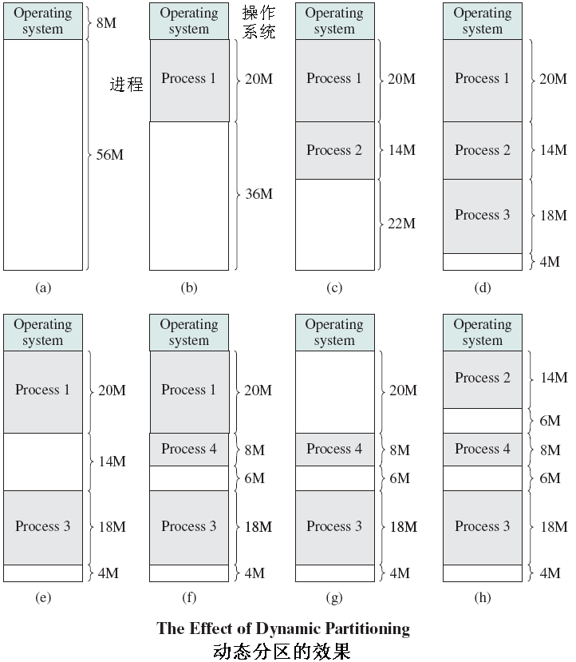
\includegraphics[width=0.6\linewidth]{fig/dynamic_partition.png}
\end{figure}

动态分区放置算法:
\begin{itemize}
    \item 首次适配(first fit):从前端开始扫描内存,直到找到一个足够大的空闲区,通常性能比较好
    \item 下次适配/邻近适配(next fit):从上次分配结束的地方开始扫描内存,直到找到一个足够大的空闲区
    \item 最佳适配(best fit)算法:扫描整个内存,找出一个足够大的最小的空闲区,会产生很多外部碎片
\end{itemize}

伙伴系统(buddy system):固定分区和动态分区的折中方案
\begin{itemize}
    \item 可用内存块大小为$2^K,L\leq K\leq U$
    \item 初始空间大小为$2^U$
    \item 若请求空间大小$s<2^{U-1}$,则对分现有块
\end{itemize}

\begin{figure}[H]
    \centering
    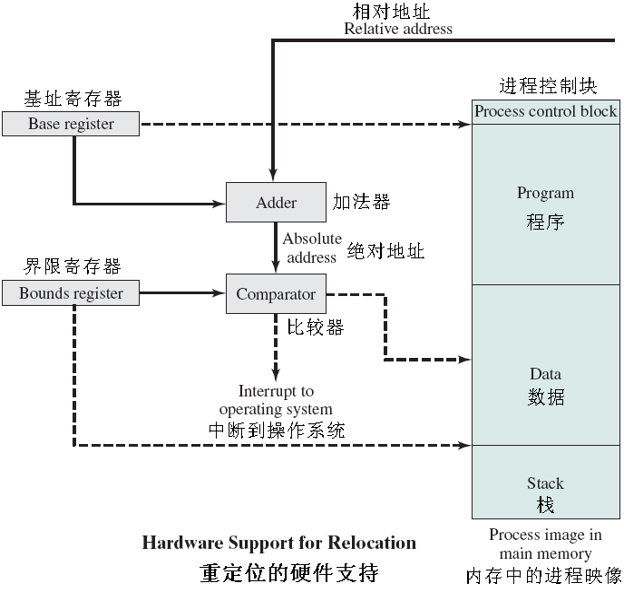
\includegraphics[width=0.5\linewidth]{fig/relocation.png}
    \caption*{重定位的硬件机制}
\end{figure}

\subsection{页式存储管理}
分页(paging)
\begin{itemize}
    \item 将主存划分为许多等长的帧/页框(frame)
    \item 将进程划分为若干页(page)
    \item 进程加载时,所有页面被载入可用帧,同时建立页表
\end{itemize}

设页大小为$L$,逻辑地址$A$,物理地址$E$,则
\[\text{页号}P=A/L\qquad\text{页内偏移量}W=A\%L\]

\begin{example}
    16位编址,若页面大小为1K(1024),则需(低)10位表示页内偏移,剩下(高)6位表示页号,则
    \begin{itemize}
        \item 相对地址为$1502$的逻辑地址$ = 1024 + 478 = (1, 478)$
        \item 逻辑地址为$(1, 478)$的相对地址$ = 1*1024 + 478 = 1502$
    \end{itemize}
\end{example}

类似固定分区,不同在于:
\begin{itemize}
    \item 分页中的“分区”(页帧)非常小(从而内碎片也小)
    \item 分页中一个进程可占用多个“分区” (页帧)(从而不需要覆盖)
    \item 分页中不要求一个进程占用的多个“分区”(页帧)连续(充分利用空闲“分区”)
\end{itemize}
存在问题:
\begin{itemize}
\item 不易实现共享和保护(不反映程序的逻辑组织)
\item 不便于动态链接(线性地址空间)
\item 不易处理数据结构的动态增长(线性地址空间)
\end{itemize}

\subsection{段式存储管理}
将程序及数据划分成若干段(segment)(不要求等长,但不能超过最大长度)
\begin{itemize}
    \item 分页是出于系统管理的需要,分段是出于用户应用的需要:
    一条指令或一个操作数可能会跨越两个页的分界处,而不会跨越两个段的分界处
    \item 页大小是系统固定的,而段大小则通常不固定
    \item 逻辑地址表示
    \begin{itemize}
    \item 分页是一维的,各个模块在链接时必须组织成同一个地址空间
    \item 分段是二维的,各个模块在链接时可以每个段组织成一个地址空间
    \end{itemize}
    \item 通常段比页大,因而段表比页表短,可以缩短查找时间,提高访问速度
    \item 分段对程序员可见,从而可用来对程序和数据进行模块化组织
    \item 分段方便实现模块化共享和保护,如程序可执行、数据可读写(段表表项要有保护位)
    \item 都存在外碎片,但分段中可通过减少段长来减轻外碎片浪费程度
    \item 分段中一个进程可占用多个“分区” ,不要求一个进程占用的多个“分区”连续(但一般要求一个段所占用的多个“分区”连续)
    \item 分段克服了分页存在的问题(数据结构的动态增长、动态链接、保护和共享)
    \item 分段存在外碎片,分页只有小的内碎片,分页内存利用率比分段高
\end{itemize}

段表只能有一个,而页表可以有多个

段页式系统中,逻辑地址被分为段号S、页号P和页内偏移量W

\subsection{虚拟存储}
传统的存储方式都是一次性加载,并且驻留在内存中。
而虚拟存储器则是基于程序的局部性原理,在程序装入时,将程序一部分装入内存,其余部分留在外存。
\begin{itemize}
    \item 采用部分加载,内存中可同时容纳更多的进程。
每个进程都只加载一部分,更多进程中应该也会有更多的就绪进程,从而提高CPU利用率
    \item 采用部分加载,进程可以比内存大,实现了虚拟存储
    \begin{itemize}
\item 用户程序可以使用的独立于物理内存的逻辑地址单元组成存储空间(虚拟存储)
\item 逻辑地址空间可以比物理地址空间大,例如,设物理内存64KB,1KB/页,则物理地址需要16位,而逻辑地址可以是28位!
\item 虚拟存储由内存和外存结合实现
    \end{itemize}
\end{itemize}

虚拟存储技术的特征:不连续性、部分交换、大空间

抖动(thrashing)问题:交换操作太过频繁

页表
\begin{itemize}
\item 页表项(Page Table Entry,简称为PTE)的一般内容:
\begin{itemize}
\item Present:在/不在内存
\item Modified:有没有被修改
\item Protection:保护码,1位或多位(rwe:读/写/执行)
\item Referenced:有没有被访问
\item Cache:是否禁止缓存
\end{itemize}
\item 页表长度不定,取决于进程大小
\item 不适合用寄存器存储页表,而是存放在内存
\item 页表起始地址保存在一个CPU专用寄存器里(\verb'cr3')
\end{itemize}

\begin{figure}[H]
    \centering
    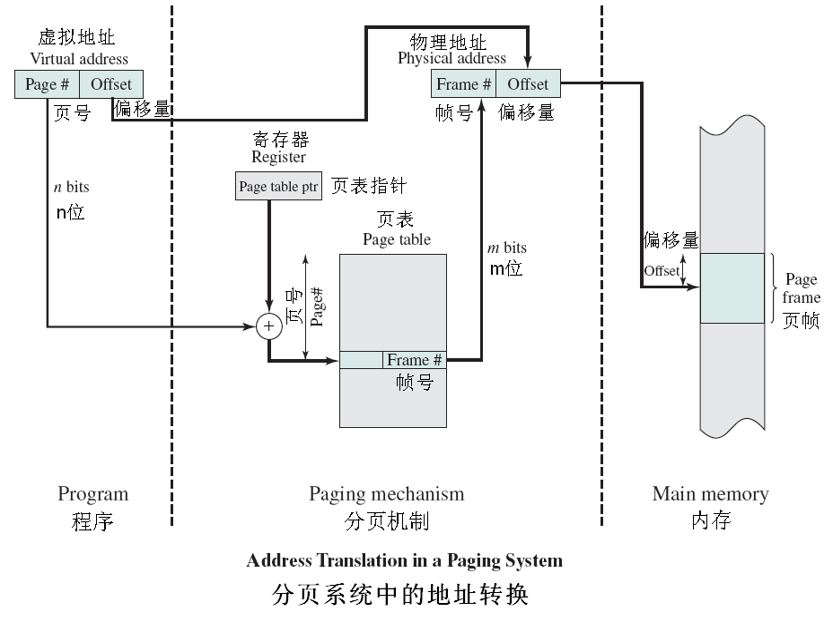
\includegraphics[width=0.8\linewidth]{fig/memory_address_transformation.png}
\end{figure}

\begin{figure}[H]
    \centering
    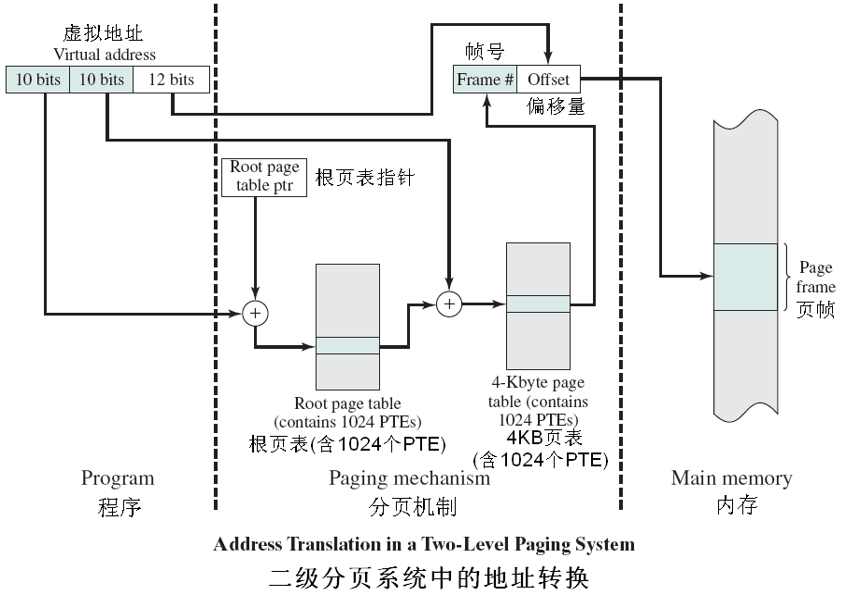
\includegraphics[width=0.8\linewidth]{fig/two-level_paging.png}
\end{figure}

快表/联想存储器(TLB)
\begin{figure}[H]
    \centering
    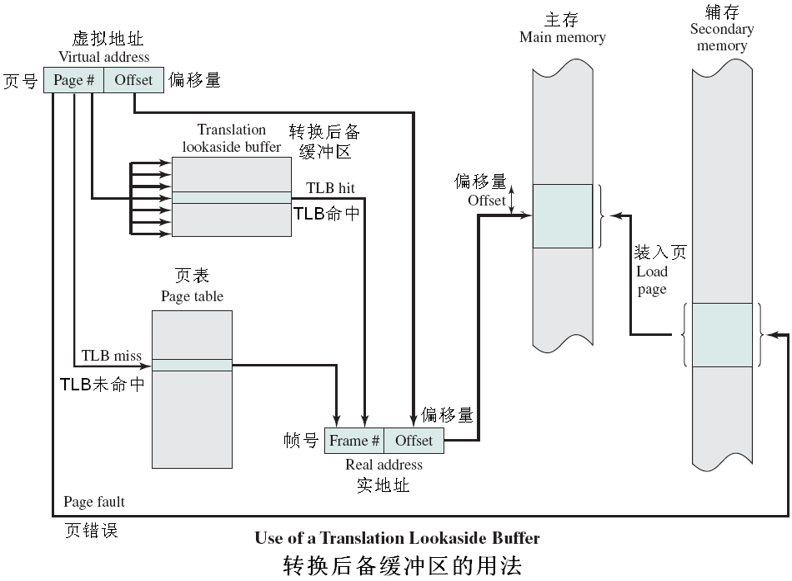
\includegraphics[width=0.8\linewidth]{fig/TLB.png}
\end{figure}

常见页面大小介于1KB-8KB

\begin{itemize}
    \item 调页策略:按需调页、预先调页
    \item 替换策略:Opt(Belady)、LRU、FIFO、Clock
\end{itemize}

Linux的内存管理
\begin{itemize}
    \item 虚拟存储采用三级页表
    \item 页面分配采用伙伴系统
    \item 页面替换采用时钟算法
\end{itemize}
% !TEX root = main.tex

\section{调度}
\subsection{单处理器调度}
\begin{itemize}
    \item 长程调度(Long-term scheduling)
    \begin{itemize}
    \item 决定哪些新建进程可进入系统准备执行
    \item 控制多道程序系统的并发程度
    \item 进程越多则各进程对CPU的使用百分比越小
    \end{itemize}
    \item 中程调度(Medium-term scheduling)
    \begin{itemize}
    \item 决定交换哪些主存-辅存(内存-外存)进程
    \item 基于多道程序设计的管理需要
    \end{itemize}
    \item 短程调度(Short-term scheduling)
    \begin{itemize}
    \item 决定下一个使用CPU的进程(dispatcher,分派程序)
    \end{itemize}
\end{itemize}

\begin{figure}[H]
    \centering
    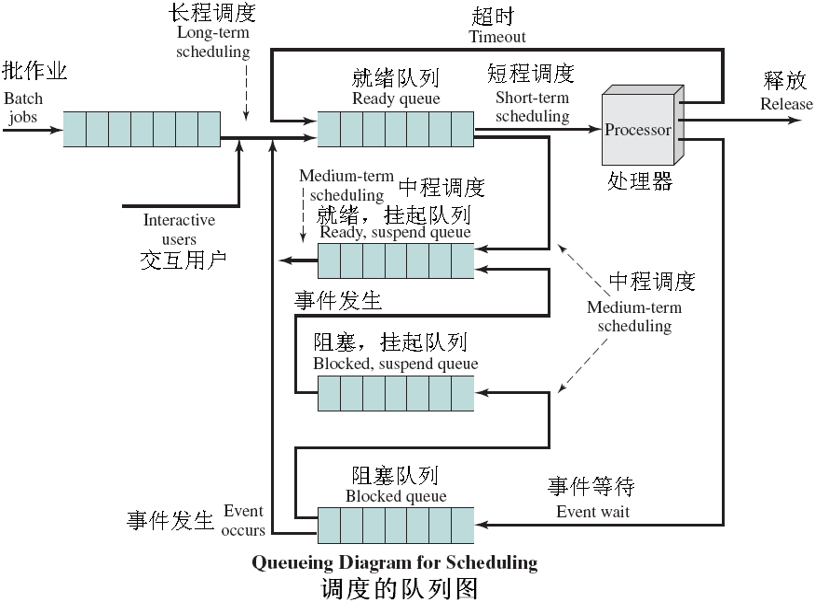
\includegraphics[width=0.8\linewidth]{fig/process_scheduling.png}
\end{figure}

进程调度算法
\begin{itemize}
\item 先来先服务(First Come First Served,FCFS)
\item 最短进程优先(Shortest Process Next,SPN):EWMA
\[S_{n+1}=aT_n+(1-a)S_n\]
\item 最短剩余优先(Shortest Remaining Time,SRT)
\item 最高响应比优先(Highest Response Ratio Next,HRRN)
\item 时间片(time slicing)轮转(Round Robin,RR)
\item 最高优先级优先(Highest Priority First,HPF)
\item 多级队列反馈(Multilevel Feedback,MF/FB)
\end{itemize}

\subsection{多处理器调度}
多处理器线程调度方案
\begin{itemize}
    \item 负载共享(load sharing)
    \item 组调度(gang scheduling)
    \item 专用处理器分配
    \item 动态调度
\end{itemize}

% 填空10*2
% 简答题6*5
% 应用题5
% !TEX root = main.tex

\section{IO管理与磁盘调度}
控制设备和内存或CPU之间的数据传送方式:
\begin{itemize}
    \item 程序控制(programmed IO)
    \item 中断驱动方式(interrupt-driven IO)
    \item 直接内存访问(Direct Memory Access, DMA)
\end{itemize}

假脱机技术(Simultaneous Peripheral Operations On Line, SPOOL)/虚拟设备技术:
专门利用一道程序来完成对设备的IO操作,而无需使用外围IO处理机
\begin{figure}[H]
    \centering
    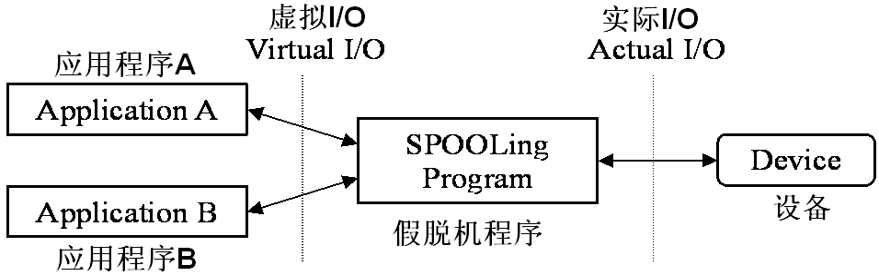
\includegraphics[width=0.7\linewidth]{fig/SPOOLing.png}
\end{figure}
优点是高速虚拟IO操作,实现对独享设备的共享

IO缓冲:
\begin{itemize}
    \item 单方向缓冲:单缓冲、双缓冲、环形缓冲
    \item 双方向缓冲:缓冲池(buffer pool)
    \item 循环缓冲
\end{itemize}

磁盘调度算法
\begin{itemize}
    \item 先进先出FIFO
    \item 优先级PRI
    \item 后进先出LIFO
    \item 最短服务时间优先(shortest-service-time-first, SSTF)
    \item 电梯算法/扫描算法SCAN
\end{itemize}
% !TEX root = main.tex

\section{文件管理}
文件目录:将所有文件控制块(File Control Block, FCB)组织在一起,一个FCB称之为一个目录项

一级目录:整个目录组织是一个线性结构,系统中所有文件都建立在一张目录表中

优缺点:
\begin{itemize}
    \item 结构简单、易实现
    \item 文件多时目录检索时间长,从而平均检索时间长
    \item 有命名冲突:如多个文件有相同的文件名或一个文件有多个不同的文件名
\end{itemize}

二级目录:在根目录/第一级目录/主文件目录MFD下,每个用户对应一个第二级目录/用户目录UFD,在用户目录下是该用户的文件,而不再有下级目录

多级目录:上下级关系
\begin{itemize}
    \item 当前目录/工作目录\verb'.'
    \item 父目录\verb'..'
    \item 子目录(subdirectory)
    \item 根目录(root directory)\verb'/'
\end{itemize}

Unix文件系统
\begin{itemize}
    \item Unix磁盘文件系统结构
    \item 引导块(块0)
    \item 超级块(块1)
    \item i-索引结点表
\end{itemize}

\begin{itemize}
\item DOS文件系统:FAT12、FAT16、FAT32
\item Windows文件系统:NTFS
\item Linux文件系统:ext2/3
\end{itemize}

\end{document}